%%% PostgreSQL Conference Europe 2013, Dublin, Oct 31, 2013
%%%
%%% A presentation of some tooling I'm building to take care of all the
%%% boring steps of the migration in a single easy and fast step: schema,
%%% handling types and default values, auto-increment and sequences, data,
%%% constraints, indexes.
%%%
%%% That feature set actually works already, only missing is a little glue
%%% and a user language to drive the tool, and that's in good progress
%%% already. The tool would definitely be ready for a full demo at the
%%% conference.
%%%
%%% Obviously the tool licence of choice is "The PostgreSQL Licence".
%%% Actually it's part of the new version of pgloader

\documentclass{beamer}

\usepackage[utf8]{inputenc}

\usepackage{beamerthemesplit}
\usetheme{Boadilla}
%\setbeamertemplate{itemize items}{\checkmark}
\setbeamertemplate{itemize items}[circle]
\beamertemplatetransparentcovered

\usepackage{multicol}

\title{From MySQL to PostgreSQL}
\subtitle{PostgreSQL Conference Europe 2013}
\author{Dimitri Fontaine \texttt{dimitri@2ndQuadrant.fr}
  \linebreak
  \url{@tapoueh}}
\date{October, 31 2013}
\logo{
\includegraphics[height=0.4cm]{2ndQuadrant-cross.png}}

\begin{document}

\frame{\titlepage}

\begin{frame}[fragile]
  \frametitle{Dimitri Fontaine}

  \begin{center}
    \textbf{2ndQuadrant France}
    \linebreak
    PostgreSQL Major Contributor
  \end{center}
  \vfill

\begin{columns}[c]
\column{.75\textwidth} 

  \begin{itemize}
   \item \texttt{pgloader}, \texttt{prefix}, \texttt{skytools}, …
   \item \texttt{apt.postgresql.org}
   \item \texttt{\textbf{CREATE EXTENSION}}
   \item \texttt{\textbf{CREATE EVENT TRIGGER}}
   \item MySQL migration tool, new \texttt{pgloader} version
  \end{itemize}  

\column{.25\textwidth}
\begin{center}
  
\includegraphics[height=7em]{2ndQuadrant-cross.png}
\end{center}
\end{columns}
\end{frame}

\section{pgloader}

\begin{frame}[fragile]
  \frametitle{Migrating from MySQL to PostgreSQL}
  
  \center{A single comand to migrate a whole database}
  \vfill

\begin{verbatim}
load database from mysql://localhost/adv
              into postgresql://dim@localhost/adv

with drop tables, truncate, create tables, create indexes,
     reset sequences,
     downcase identifiers
 set work_mem to '128MB', maintenance_work_mem to '512 MB'

cast type datetime to timestamptz drop default using zero-dates-to-null,
     type date drop not null drop default using zero-dates-to-null,
     type tinyint to boolean using tinyint-to-boolean;
\end{verbatim}
\end{frame}

\begin{frame}[fragile]
  \frametitle{Migrating from MySQL to PostgreSQL}
  
  \center{TODO: prepare a real test case}
  \vfill

\begin{verbatim}
        table name   imported     errors       time
------------------  ---------  ---------  ---------
           extract          0          0      2.046
       before load          0          0      0.032
------------------  ---------  ---------  ---------
  geolite.location     438386          0      9.194
    geolite.blocks    1790461          0     18.021
------------------  ---------  ---------  ---------
           finally          0          0     31.593
------------------  ---------  ---------  ---------
 Total import time    2228847          0   1m0.886s
\end{verbatim}
\end{frame}

\section{Why}

\begin{frame}[fragile]
  \frametitle{Why Migrating from MySQL to PostgreSQL?}
  
  \center{Migrating is a costly process, why doing it?}
  \vfill

\begin{columns}[c]
\column{.5\textwidth} 

  \center{MySQL}

  \begin{itemize}
  \item Storage Engine
  \item Single Application
  \item Data Loss with Replication
  \item Weak Data Types Validation
  \item Either transactions or
  \item Loack of
  \end{itemize}

\column{.5\textwidth} 

  \center{PostgreSQL}

  \begin{itemize}
  \item Data Access Service
  \item Application Suite
  \item Durability and Availability
  \item Consistency
  \item Full Text Search, PostGIS
  \item Documentation
  \end{itemize}
\end{columns}
\end{frame}

\begin{frame}[fragile]
  \frametitle{Free your Data!}

\begin{center}
  
\includegraphics[height=18em]{free-our-open-data.jpg}
\end{center}
\end{frame}

\begin{frame}[fragile]
  \frametitle{Cost Analysis}
  
  \center{What are the costs?}
  \vfill

\begin{columns}
\column{.6\textwidth}

  \begin{itemize}
  \item Migrating the Data
  \item Migrating the Code
  \item Quality Assurance
  \item Opportunity Cost
  \end{itemize}  

\column{.4\textwidth}
\begin{center}
  
\includegraphics[height=7em]{Dollar-sign.jpg}
\end{center}
\end{columns}
\end{frame}

\section{How}

\begin{frame}[fragile]
  \frametitle{How pgloader migrates your data}
  
  \center{pgloader Architecture Choices and features}
  \vfill

\begin{columns}
\column{.6\textwidth}

  \begin{itemize}
  \item Streaming with the COPY protocol
  \item Asynchornous IO with Threads
  \item User Editable Casting Rules
  \item Transforms
  \end{itemize}  

\column{.4\textwidth}
\begin{center}
  TODO: PICTURE
\end{center}
\end{columns}
\end{frame}

\begin{frame}[fragile]
  \frametitle{How pgloader migrates your data}
  
  \center{User Editable Casting Rules}
\end{frame}

\begin{frame}[fragile]
  \frametitle{How pgloader migrates your data}
  
  \center{Transforms}
\end{frame}

\begin{frame}[fragile]
  \frametitle{pgloader limitations}
  
  \center{The 80\% rule}
  \vfill

  \begin{itemize}
  \item Views
  \item Triggers
  \item Foreign Keys
  \item \texttt{ON UPDATE CURRENT\_TIMESTAMP}
  \item Geometric datatypes
  \item Per Column Casting Rules
  \end{itemize}
\end{frame}

\section{Conclusion}

\begin{frame}
  \frametitle{Questions?}

\begin{center}
  Now is the time to ask!
  \vfill

  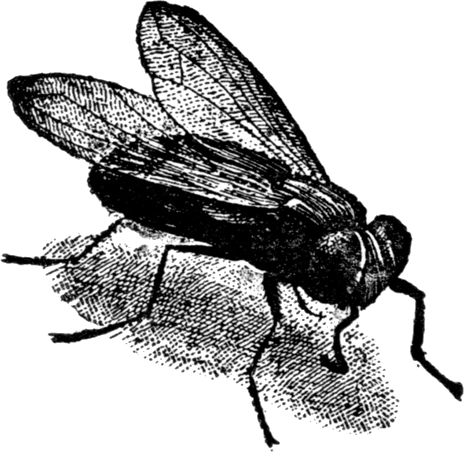
\includegraphics[height=9em]{fly.png}
\end{center}
\end{frame}

\end{document}
